\documentclass[a4paper,12pt]{article}

% Encodage
\usepackage[utf8]{inputenc}
\usepackage[T1]{fontenc}
\usepackage[french]{babel}

% Mise en page
\usepackage{geometry}
\geometry{margin=2.5cm}

% Gestion des espaces et tableaux
\usepackage{graphicx}   % pour les images
\usepackage{array}      
\usepackage{ragged2e}   
\renewcommand\labelitemi{$\bullet$}
\begin{document}
\begin{center}
    {\LARGE \textbf{CURRICULUM VITAE}}
\end{center}
\noindent
\begin{minipage}{0.45\textwidth}
    \raggedright
    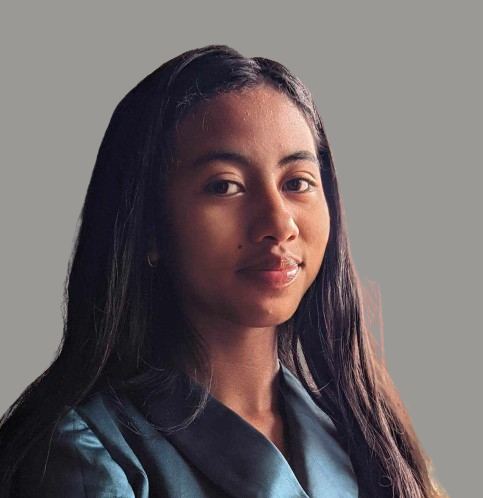
\includegraphics[width=6cm]{faniriana_cv.png} \\[0.5cm]
\end{minipage}
\hfill
\begin{minipage}{0.45\textwidth}
    \raggedright
    {\LARGE \textbf{VOAHARIMPITIAVANA}} \\[0.2cm]
     \textbf{Andraina Faniriana}\\[0.8cm]
     {\LARGE \textbf{Data analyst}}
\end{minipage}

\vspace{0.5cm} % espace vertical après les minipages
\begin{minipage}{0.45\textwidth}

\end{minipage}
\noindent

\textbf{Profil :} \\[0.3cm]
Étudiante passionnée par l’analyse de données, motivée et autodidacte, je maîtrise les bases de la programmation et de la visualisation, avec pour objectif de contribuer à des projets concrets en tant que Data Analyste junior.\\[0.4cm]
\begin{minipage}{0.45\textwidth}
    \raggedright
\textbf{Compétence :} \\
\begin{itemize}
    \renewcommand\labelitemi{$\bullet$} % puce en point
    \item{ \textbf{Analyse de données : }Nettoyage, transformation, exploration des données}
    \item{ \textbf{Langages : }Python (Pandas, NumPy, Matplotlib, Seaborn), SQL, R}
    \item{ \textbf{Outils : }Excel, Power BI, Tableau, Jupyter Notebook}
    \item{ \textbf{Base de données : }MySQL, PostgreSQL}
    \item{ \textbf{Compétences transversales : }Rigueur, curiosité, esprit analytique, autonomie}
\end{itemize}
\vspace{0.3cm}
\textbf{Formation :} \\
\begin{itemize}
    \renewcommand\labelitemi{$\bullet$} % puce en point
        \item{ \textbf{Licence en cours : }Université de INSI
        }
        \item{ \textbf{Cours en ligne et Certifications de donnée en cours : }Google Cloud Skill Boost
        }
\end{itemize}
\end{minipage}
\hfill
\vrule width 0.5pt % épaisseur du trait vertical
\hfill
\begin{minipage}{0.45\textwidth}
\raggedright
\vspace{0.5cm}
\textbf{Projets académiques et personnels :}\\
\begin{itemize}
\renewcommand\labelitemi{$\bullet$} % puce en point
    \item{ \textbf{Analyse des facteurs associés au turnover des employés : }
        \begin{itemize}
        \renewcommand\labelitemi{$\bullet$} % puce en point
            \item{ dashboard turnover par département, fonction, niveau d'étude, ancienneté avec Power BI. 
            }
            \item{ 
            Visualisation des départs et tendances, classification des employés
            }
        \end{itemize}
        }
        
    \item{ \textbf{traitement de AmesHousing : }
        \begin{itemize}
        \renewcommand\labelitemi{$\bullet$} % puce en point
            
            \item{ nettoyage et normalisation du donnée.
            }
            \item{ Prediction de prix de vente des maisons). 
            }
        \end{itemize}
    }
    \end{itemize}
    \vspace{0.5cm}
\textbf{Langues :}\\
\begin{itemize}
    \renewcommand\labelitemi{$\bullet$} % puce en point
        \item{ \textbf{Français : }}intermédiaire
        \item{  \textbf{Anglais : }}advanced (technical and business)
        \item{  \textbf{Malagasy : }}langue maternelle
\end{itemize}
        
\end{minipage}
\end{document}
